\documentclass[12pt,twocolumn,oneside]{osajnl}
%% Please use 11pt if submitting to AOP
%\documentclass[14pt,twocolumn,twoside]{osajnl}

\journal{ao} % Choose journal (ao, aop, josaa, josab, ol, pr)

% See template introduction for guidance on setting shortarticle option
\setboolean{shortarticle}{true}
% true = letter / tutorial
% false = research / review article
% (depending on journal).

\title{An Approach To The Traveling Salesman Problem Using A Hybrid Genetic Algorithm}

%\author{E Garg}
%\author{S Parson}
%\author{T Rahman}
\author{E Garg, S Parson, T Rahman, J Wagner}

%\affil[1]{Publications Department, The Optical Society (OSA), 2010 Massachusetts Avenue NW, Washington D.C., 20036}
%\affil[2]{School of Science, University of Technology, 2000 J St. NW, Washington DC, 20036}
%\affil[3]{School of Optics, University of Technology, 2000 J St. NW, Washington DC, 20036}

%\affil[*]{Corresponding author: email@my-email.com}

%% To be edited by editor
% \dates{Compiled \today}

%\ociscodes{(140.3490) Lasers, distributed feedback; (060.2420) Fibers, polarization-maintaining;(060.3735) Fiber Bragg gratings.}

%% To be edited by editor
% \doi{\url{http://dx.doi.org/10.1364/XX.XX.XXXXXX}}

\begin{abstract}
This paper explores the application and performance testing of a hybrid genetic algorithm implemented in Python. Variations of crossover and mutation are compared in a battle for fastest time to (near) convergence. The results shed a light on the nature of the search space and a better understanding of the fitness landscape's multitude of local (near-optimal) minima.  There is potential for improvement for this algorithm, especially in regards to changing parameters as we plateau. It can be inferred that there is a need for reinforcement learning to exit deep local minima, however the performance of the algorithm is acceptably close to optimum. 
\end{abstract}

\setboolean{displaycopyright}{false}

\begin{document}

\maketitle

\section{Introduction}
Mathematically described as the shortest Hamiltonian circuit, the Traveling Salesman Problem describes the problem of determining the shortest path length of a weighted graph traversal of $n$ nodes with the constraint that the start and end node are the same. The problem was tested on a data set consisting of three real-world instances of the problem, namely graphs derived from maps of the Western Sahara, Uruguay, and Canada. These instances consist of 29, 734, and 4663 nodes respectively.

Since each path is a ordered set of nodes, the chosen representation is a sequence whose non-repeating elements consist of each node visited, in the path order. This sequential set is hereafter referred to as the \textit{chromosome} to make the relationship to genetic crossover and mutation more apparent. 

Representing the path this way is very compact, and can represent any solution path. A tree could be an alternative representation, however this would introduce an extra layer of complexity into the problem. One key aspect of a representation is that it must be able to express our target solution, which is an evident characteristic.

 There exists a positive correlation between the number of nodes and the computational complexity of the problem. The search space of this representation grows as an unbounded monotonic factorial function. For the Western Sahara data set, there are $3.05x10^{29}$ solutions alone. Uruguay has only twenty-five times as many cities, however the search space has $4.12x10^{1783}$ solutions. The situation is even bleaker for the Canada set, which has a whopping $2.73x10^{15080}$ solutions.

\section{Methodology}
\label{sec:methodology}
A genetic algorithm has a number of elements that make variants unique from each other. Each algorithm has an initialization procedure, evaluation function, parent selection methodology, recombination operator(s), mutation operator(s), and survivor selection methodology. Each of these will be described in the following sections.
\subsection{Initialization: Clustering}

As previously discussed, the search space for this problem is enormously large. Even with the smallest data set, brute-force search on the Western Sahara data set would require $3.05x10^{29}$ evaluations to find the optimal solution. Assuming that we are able to evaluate one solution every microsecond, it would still take 100,000,000,000,000 \textit{centuries} to exhaustively evaluate every solution.

There is a strong need to remove unlikely candidates from the solution space. One method to reduce the number of solutions is to group nearby nodes into individual \textit{clusters}. 

Being one of the most popular clustering algorithms, \textit{k-means clustering} was chosen the organize the nodes. Given a number \textit{k}, all the nodes are separated into \textit{k} clusters. Each cluster has a node that acts as the centre of the cluster. Then, the algorithm iterates over each node and assigns it to the cluster with the centre node that it is closest to. Conceptually, it can be thought of as dividing the TSP problem into smaller TSP sub-problems\cite{hartigan1979algorithm} \cite{wilkin2007k}. The algorithm can be concisely expressed as the following series of steps:

\begin{enumerate}
    \item Given a number \textit{k}, randomly pick \textit{k} cities that will act as cluster centres.
    \item For every city \textit{C}:
    \begin{enumerate}
        \item Calculate the distance between \textit{C} and every cluster centre city.
        \item Pick the cluster with the centre that is closest to \textit{C}.
        \item Add the city \textit{C} to that cluster.
    \end{enumerate}  
    \item For every cluster$^{*}$:
    \begin{enumerate}
        \item For every city \textit{$C_1$}, calculate the cumulative distance between itself and every other city in the cluster.
        \item Pick the city with the smallest cumulative distance to every other city and assign it to be the new centre of the current cluster.
        \item Repeat \textbf{Step 3} \textit{n} times (where \textit{n} is specified in advance).
    \end{enumerate}
    \item Now that the clusters have been established, order all the clusters by their centres, so that the closest clusters stay close to each other.
\end{enumerate}

$^{*}$Step 3 is usually performed until the clusters become static. Due to computational limitations, we decided that it is better to constrain the number of iterations for \textbf{Step 3} to \textit{n} (where \textit{n} is specified in advance in the configuration).

\subsection{Evaluation}
As discussed previously, our population is modeled as instances of orderings. This representation can be evaluated simply by adding together the weights of every consecutive pair of edges of the node pair. The calculation will yield a sum, which is to be minimized. The weights between all pairs of nodes have been added to a two-dimensional array, ensuring that this addition is a constant-time operation.

\subsection{Parent Selection}
Tournament selection was the method of choice for parent selection. It was chosen due to the fact that it adds an extra element of randomness to the algorithm to try to combat the problem of reaching local minima. It involves the following steps:

\begin{enumerate}
    \item Pick $k$ individuals randomly, without replacement.
    \item Out of these $k$ individuals, select the individual with the best fitness and add it to the mating pool.
    \item Repeat until a mating pool of the desired size is obtained.
\end{enumerate}

\subsection{Recombination}
To perform crossover between chromosomes, two operators were implemented and compared. The first of which, called \textit{cut-and-crossfill} is implemented, which is then compared to a newer method called \textit{best-order}.

\textbf{Cut-And-Crossfill}: As described in Eiben's book, cut-and-crossfill is a relatively simple algorithm for recombining two chromosomes into a pair of chromosomes, using information from both parent chromosomes\cite{eiben2008introduction}.

The algorithm can be concisely expressed as the following series of steps:
\begin{enumerate}
    \item Define a new empty arrays $o_1$ and $o_2$
    \item Choose a random point $j$ on the interval $[1, k-1]$ where $k$ is the length of the chromosome.
    \item Copy elements $[0, j]$ from the first parent into $o_1$
    \item Append to $o_1$ the elements $[j+1, k]$ of the first parent
    \item Copy elements $[0, j]$ from the second parent into $o_2$
    \item Append to $o_2$ the elements $[j+1, k]$ of the second parent
\end{enumerate}

The algorithm's ease-of-implementation and computational speed make it the algorithm of choice to compare to newer, more complicated operators.

\textbf{Best-Order Crossover}: Best-order crossover is predicated on the assumption that the order of the alleles is more important than their positions. This operator incorporates genetic material from the current best chromosome in the population along with the genetic material from the two parent chromosomes participating. Thus, the order of particular genes in the offspring can be informed by the order of those genes in the best individual chromosome present in the population\cite{andreica2015best}.

In the current problem context, the information describing the order of alleles with respect to each other is more important than a particular allele being present in a specific location, since there is no restriction on the starting position.

The Best Order Crossover operator involves the following steps:
\begin{enumerate}
    \item Pick $n$ random crossover points, resulting in $n+1$ sub-sequences of specified minimum length.
    \item For each resulting sub-sequence:
    \begin{enumerate}
        \item Generate a random integer between $r$, where $1 <= r <= 3$.
        \item If $r == 1$, then the alleles corresponding to this subsequence will be taken from Parent 1 in the order that they are in Parent 1.
        \item If $r == 2$, then the alleles corresponding to this subsequence will be taken from Parent 1, but in the order that they appear in Parent 2.
        \item If $r == 3$, then the alleles corresponding to this subsequence will be taken from Parent 1, but in the order that they appear in the best individual in the current generation.
    \end{enumerate}
\end{enumerate}

\subsection{Mutation}
For mutation, we used permutation swap, insertion mutation, inversion mutation, scramble mutation, two-opt mutation and a cyclic “random” mutation operator.

\textbf{Permutation Swap}: This operator picks two random alleles in the chromosome and swaps their positions.

\textbf{Insertion Mutation}: This operator involves the following steps:
\begin{enumerate}
    \item Pick two random alleles $n_1$ and $n_2$
    \item Insert $n_1$ adjacent to $n_2$
\end{enumerate}

\textbf{Inversion Mutation}: This mutation operator picks two random alleles in the chromosome and inverts (reverses) the sub-sequence of alleles between them. The length of the sub-sequence to be inverted/reversed can be specified in advance.

\textbf{Scramble Mutation}
For this mutation operator, two random alleles in the chromosome are chosen and the sub-sequence of alleles between them are scrambled. The length of the sub-sequence to be scrambled can be specified in advance.

\textbf{2-Opt Swap Mutation}
This operator was inspired by the 2-opt local search algorithm, which is often employed to solve this problem class.  This mutation operator picks two adjacent pairs of alleles and swaps their respective elements\cite{croes1958method}.

This operator involves the following steps:

\begin{enumerate}
    \item Pick a random alleles $n_1$ and $n_3$
    \item Choose $n_2$ such that it is an arbitrarily adjacent node to $n_1$, and likewise choose a $n_4$ adjacent to $n_3$.
    \item Treat the four alleles as adjacent pairs, where the first pair is ($n_1$, $n_2$) and the second pair is ($n_3$, $n_4$).
    \item Swap the elements the pairs with each other.
\end{enumerate}


\textbf{Cyclic Random Mutation}
An operator was devised that randomly picks a mutation operator out the aforementioned operators. The idea was that different operators are helpful for getting out of different types of local minima.

\subsection{Survivor Selection}
We used ($\mu$ + $\lambda$) selection for survivor selection, which involves the following steps:

\begin{enumerate}
    \item Pool all $\mu$ current generation individuals and $\lambda$ offspring together.
    \item Rank them by fitness
    \item Pick the top $\mu$ individual to enter the next generation
\end{enumerate}



\section{Discussion}
For all results in this section, the Uruguay data set was used as the basis of comparison, with all other parameters of the algorithm held constant, other than the parameter under test. These parameters are expressed in Table \ref{tab:parameters}. Uruguay was chosen due to the fact that the solution space is very large and the we can perform a run of this algorithm in a manageable amount of time.
\begin{table}[htbp]
\centering
\caption{\bf Parameters Of The Hybrid Genetic Algorithm}
\begin{tabular}{ccc}
\hline
Parameter & Value \\
\hline
Data Source && $TSP\_Uruguay\_734.txt$ \\
Pop. Size && $20$ \\
Init. Method && $k-means$ \\
Mating Pool Size && $10$ \\
Tournament Size && $5$ \\
Crossover Rate && $90\%$ \\
Mutation Rate && $80\%$ \\
Generations && $1000$ \\
BOX Cutting Points && $240$ \\
K-Means Clusters && $220$ \\
K-Means Iterations && $5$ \\


\hline
\end{tabular}
  \label{tab:parameters}
\end{table}



\subsection{Smart Initialization}
While the k-means clustering algorithm reduces the search space substantially, it does so by yielding a deep local minima. This local minima can reach as close to 113\% of the optimal solution, which is very close to the optimum result. After the clusters of nodes are defined, there is a need to order them in their own Hamiltonian cycle, which is basically a smaller version of the TSP problem. Augmenting the k-means algorithm to properly order the initial clusters will yield even better results. The hybrid algorithm results in good quality solutions in a minimal number of generations. Without the clustering, the algorithm starts at a much worse fitness value, as evidenced by Figure \ref{fig:kmeans}. The difference is substantial, in that random initialization resulted in a mean starting fitness of 1,579,829, whereas k-means was 121,647, an order of magnitude better.

\begin{figure}[htbp]
\centering
\fbox{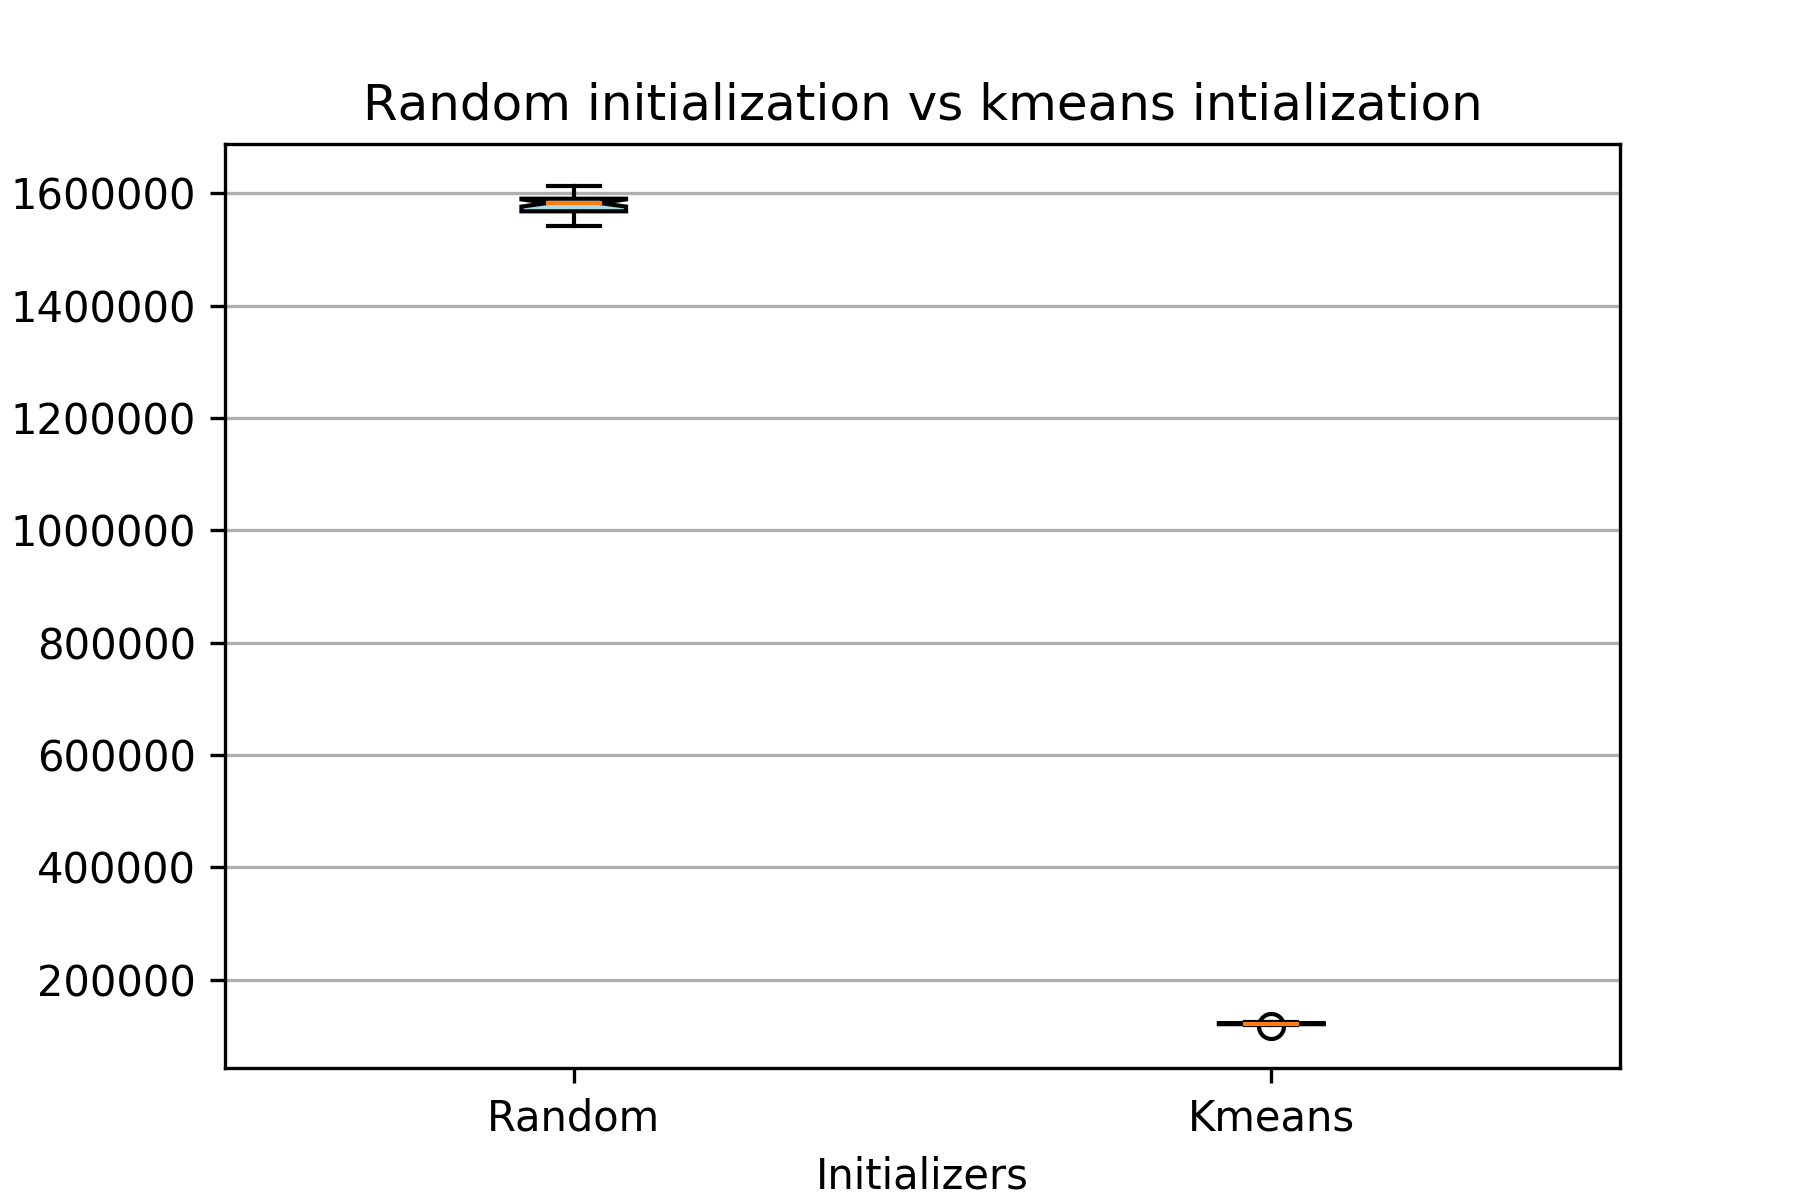
\includegraphics[width=\linewidth]{boxplot.png}}
\caption{Boxplots indicating the distribution of initial fitnesses using both kmeans and random initialization.}
\label{fig:kmeans}
\end{figure}

\subsection{Crossover}
Figure \ref{fig:bovcc} alludes to the idea that the mean fitness values are lower (better) for best-order crossover compared to cut-and-crossfill. 

Plotting a notched boxplot in Figure \ref{fig:bovboxplot}, it is evident that the confidence intervals are nearly stacked end to end, in favor of best-order crossover. It is noteworthy that there are no outliers in each set, and the range is similar in each case.

Figure \ref{fig:bocchist} plots the histogram of each run. It is not apparent that the samples are normally distributed, so we have chosen the Mann-Whitney-U test as the statistical test of choice, since it does not require the assumption of normality.

For each crossover algorithm, thirty runs were conducted with all other parameters remaining constant. A one-tailed Mann-Whitney-U test to test the null hypothesis that cut-and-crossfill has a mean best fitness equal to or smaller than best-order crossover. Obtaining a p-value of 0.0099, we reject the aforementioned null hypothesis. The alternative hypothesis is accepted, favoring the best-order crossover with 95\% confidence.

\begin{figure}[htbp]
\centering
\fbox{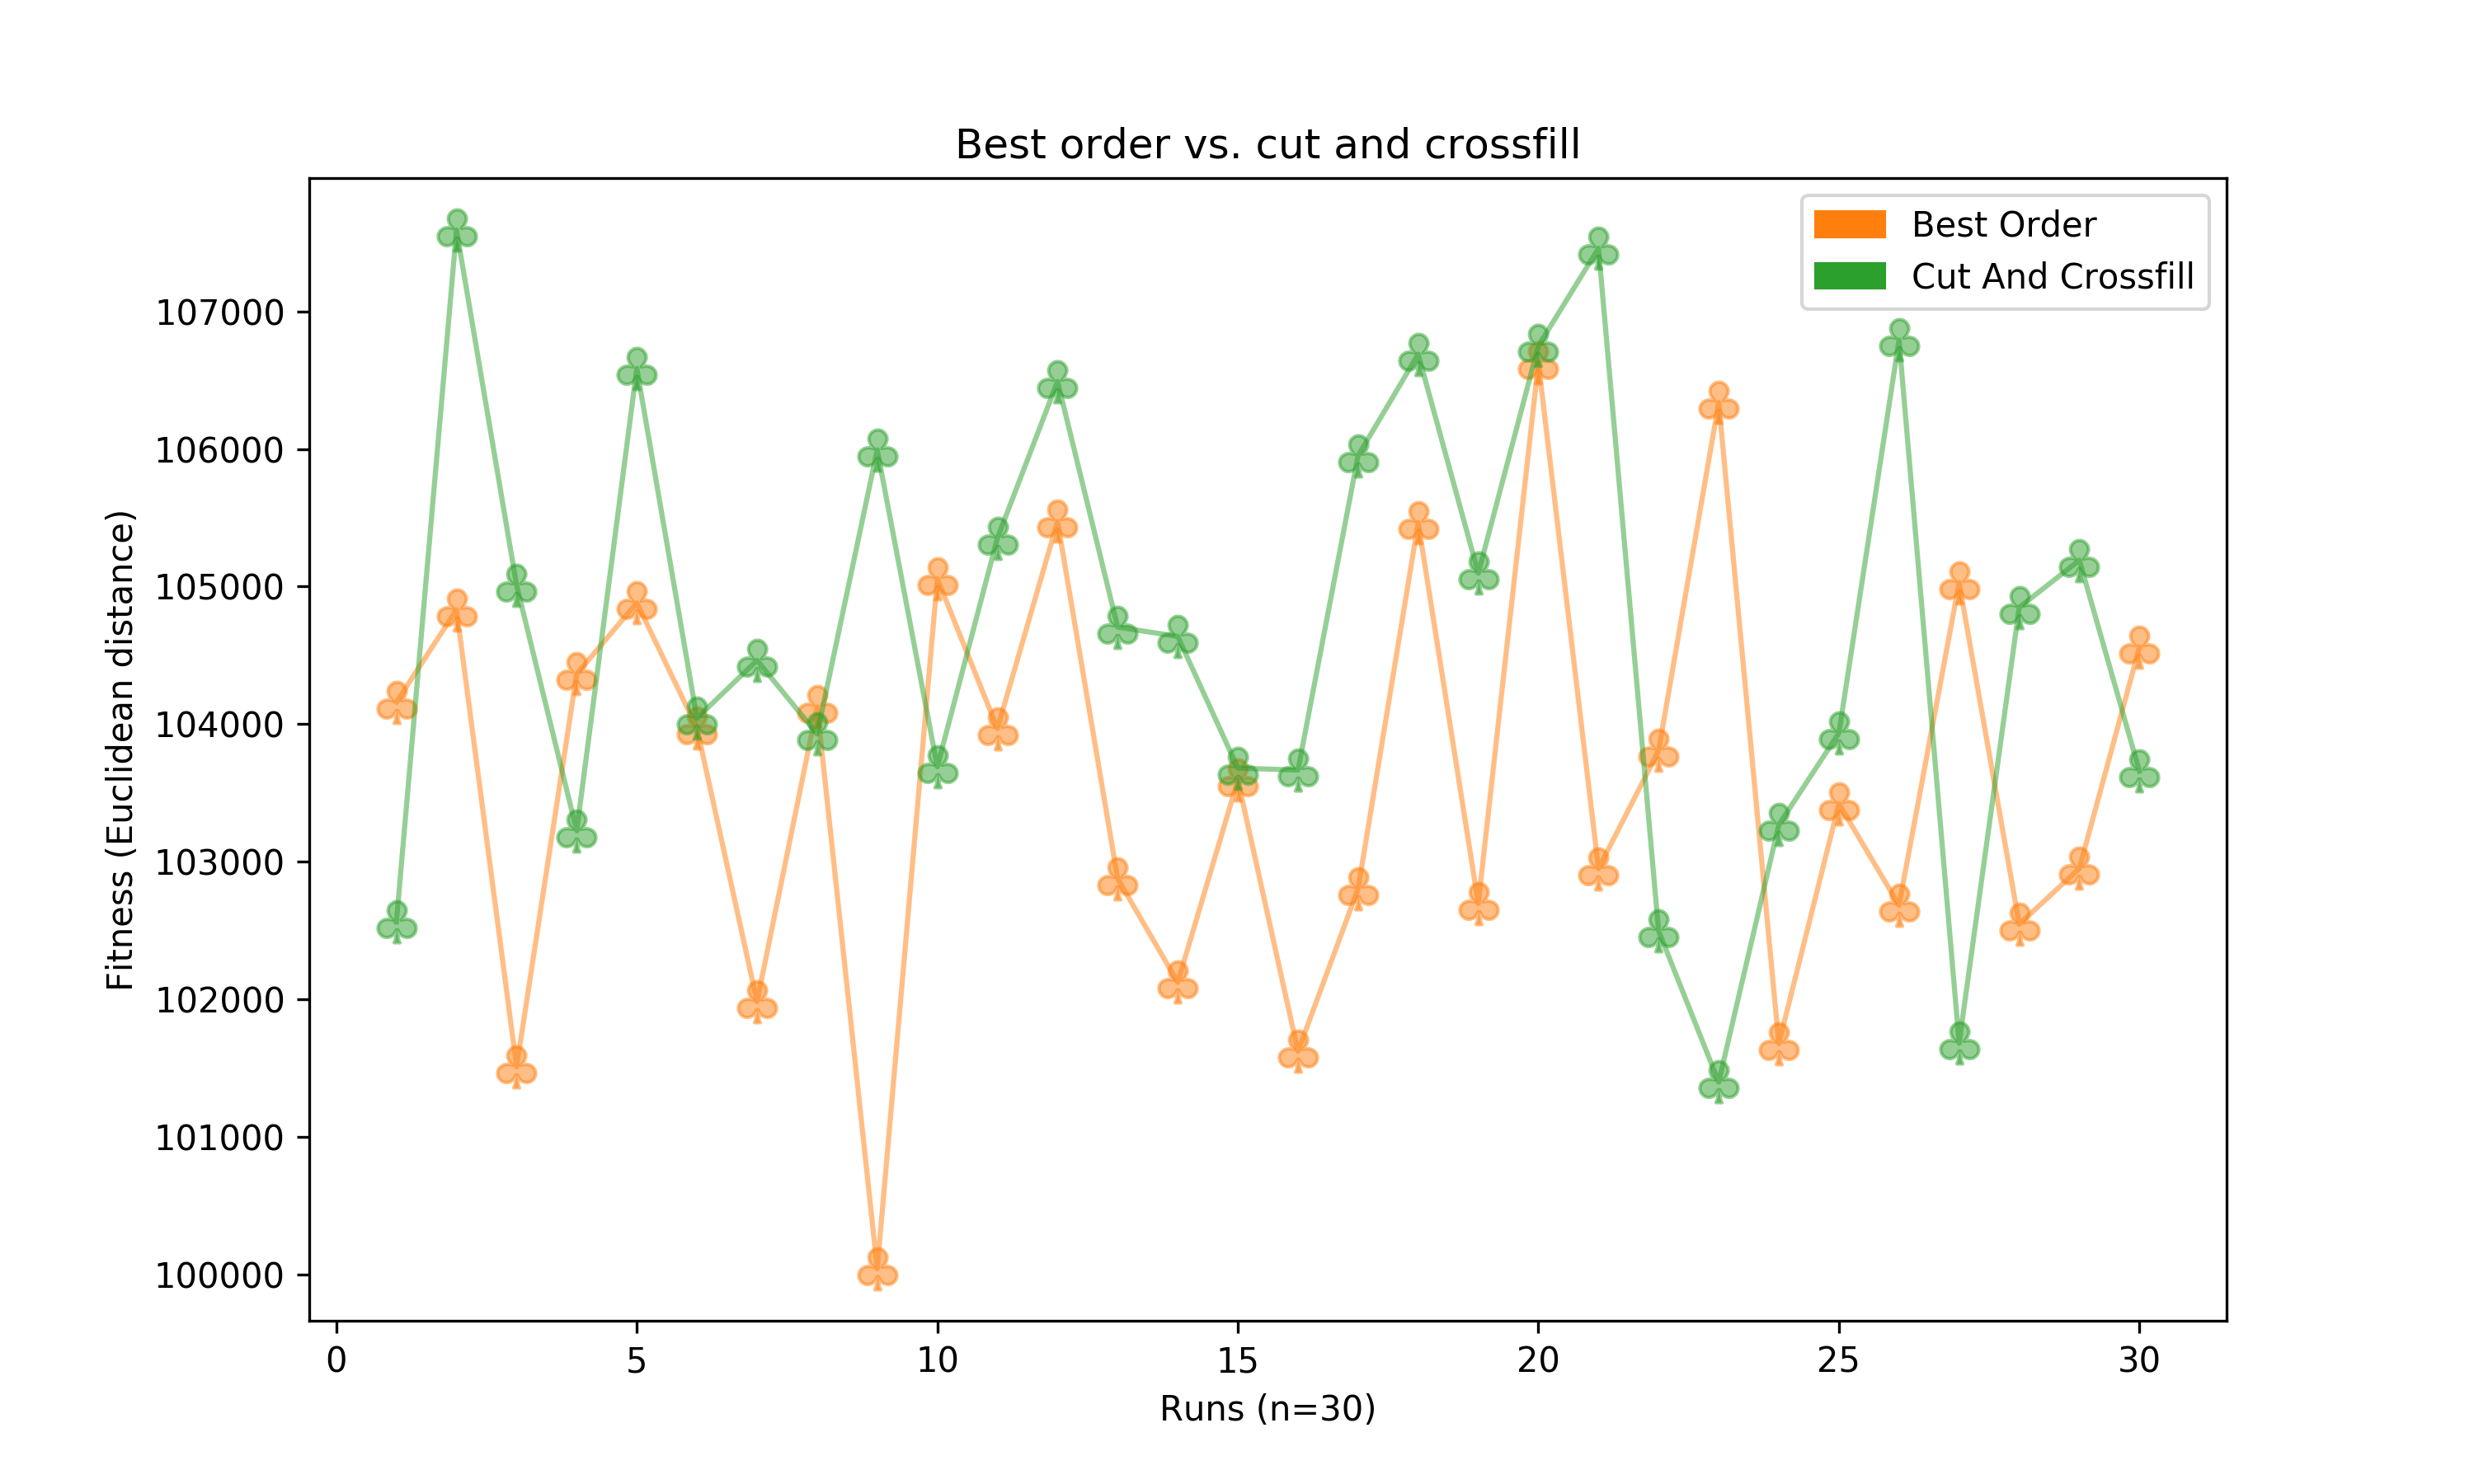
\includegraphics[width=\linewidth]{bovcc.png}}
\caption{Comparison of the mean best fitness of best-order vs. cut-and-crossfill crossover consisting of thirty runs each.}
\label{fig:bovcc}
\end{figure}

\begin{figure}[htbp]
\centering
\fbox{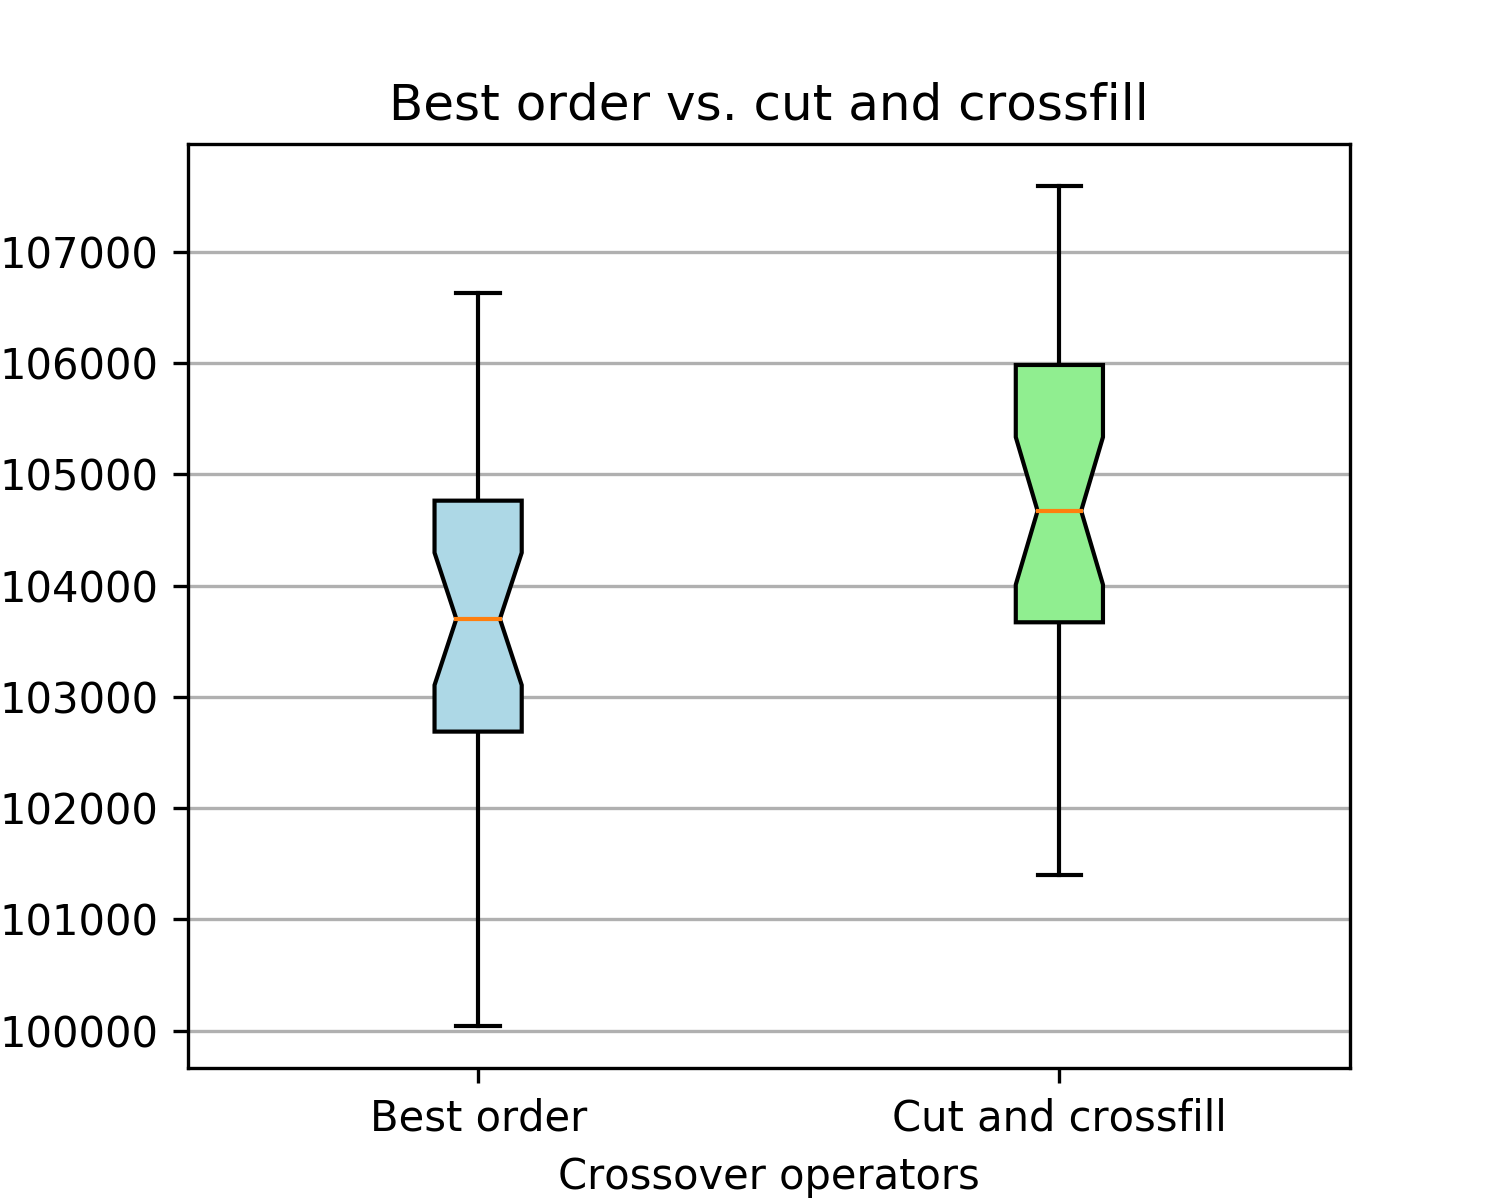
\includegraphics[width=\linewidth]{boccboxplot.png}}
\caption{Notched boxplots of the best fitnesses of best-order vs cut-and-crossfill crossover.}
\label{fig:bovboxplot}
\end{figure}

\begin{figure}[htbp]
\centering
\fbox{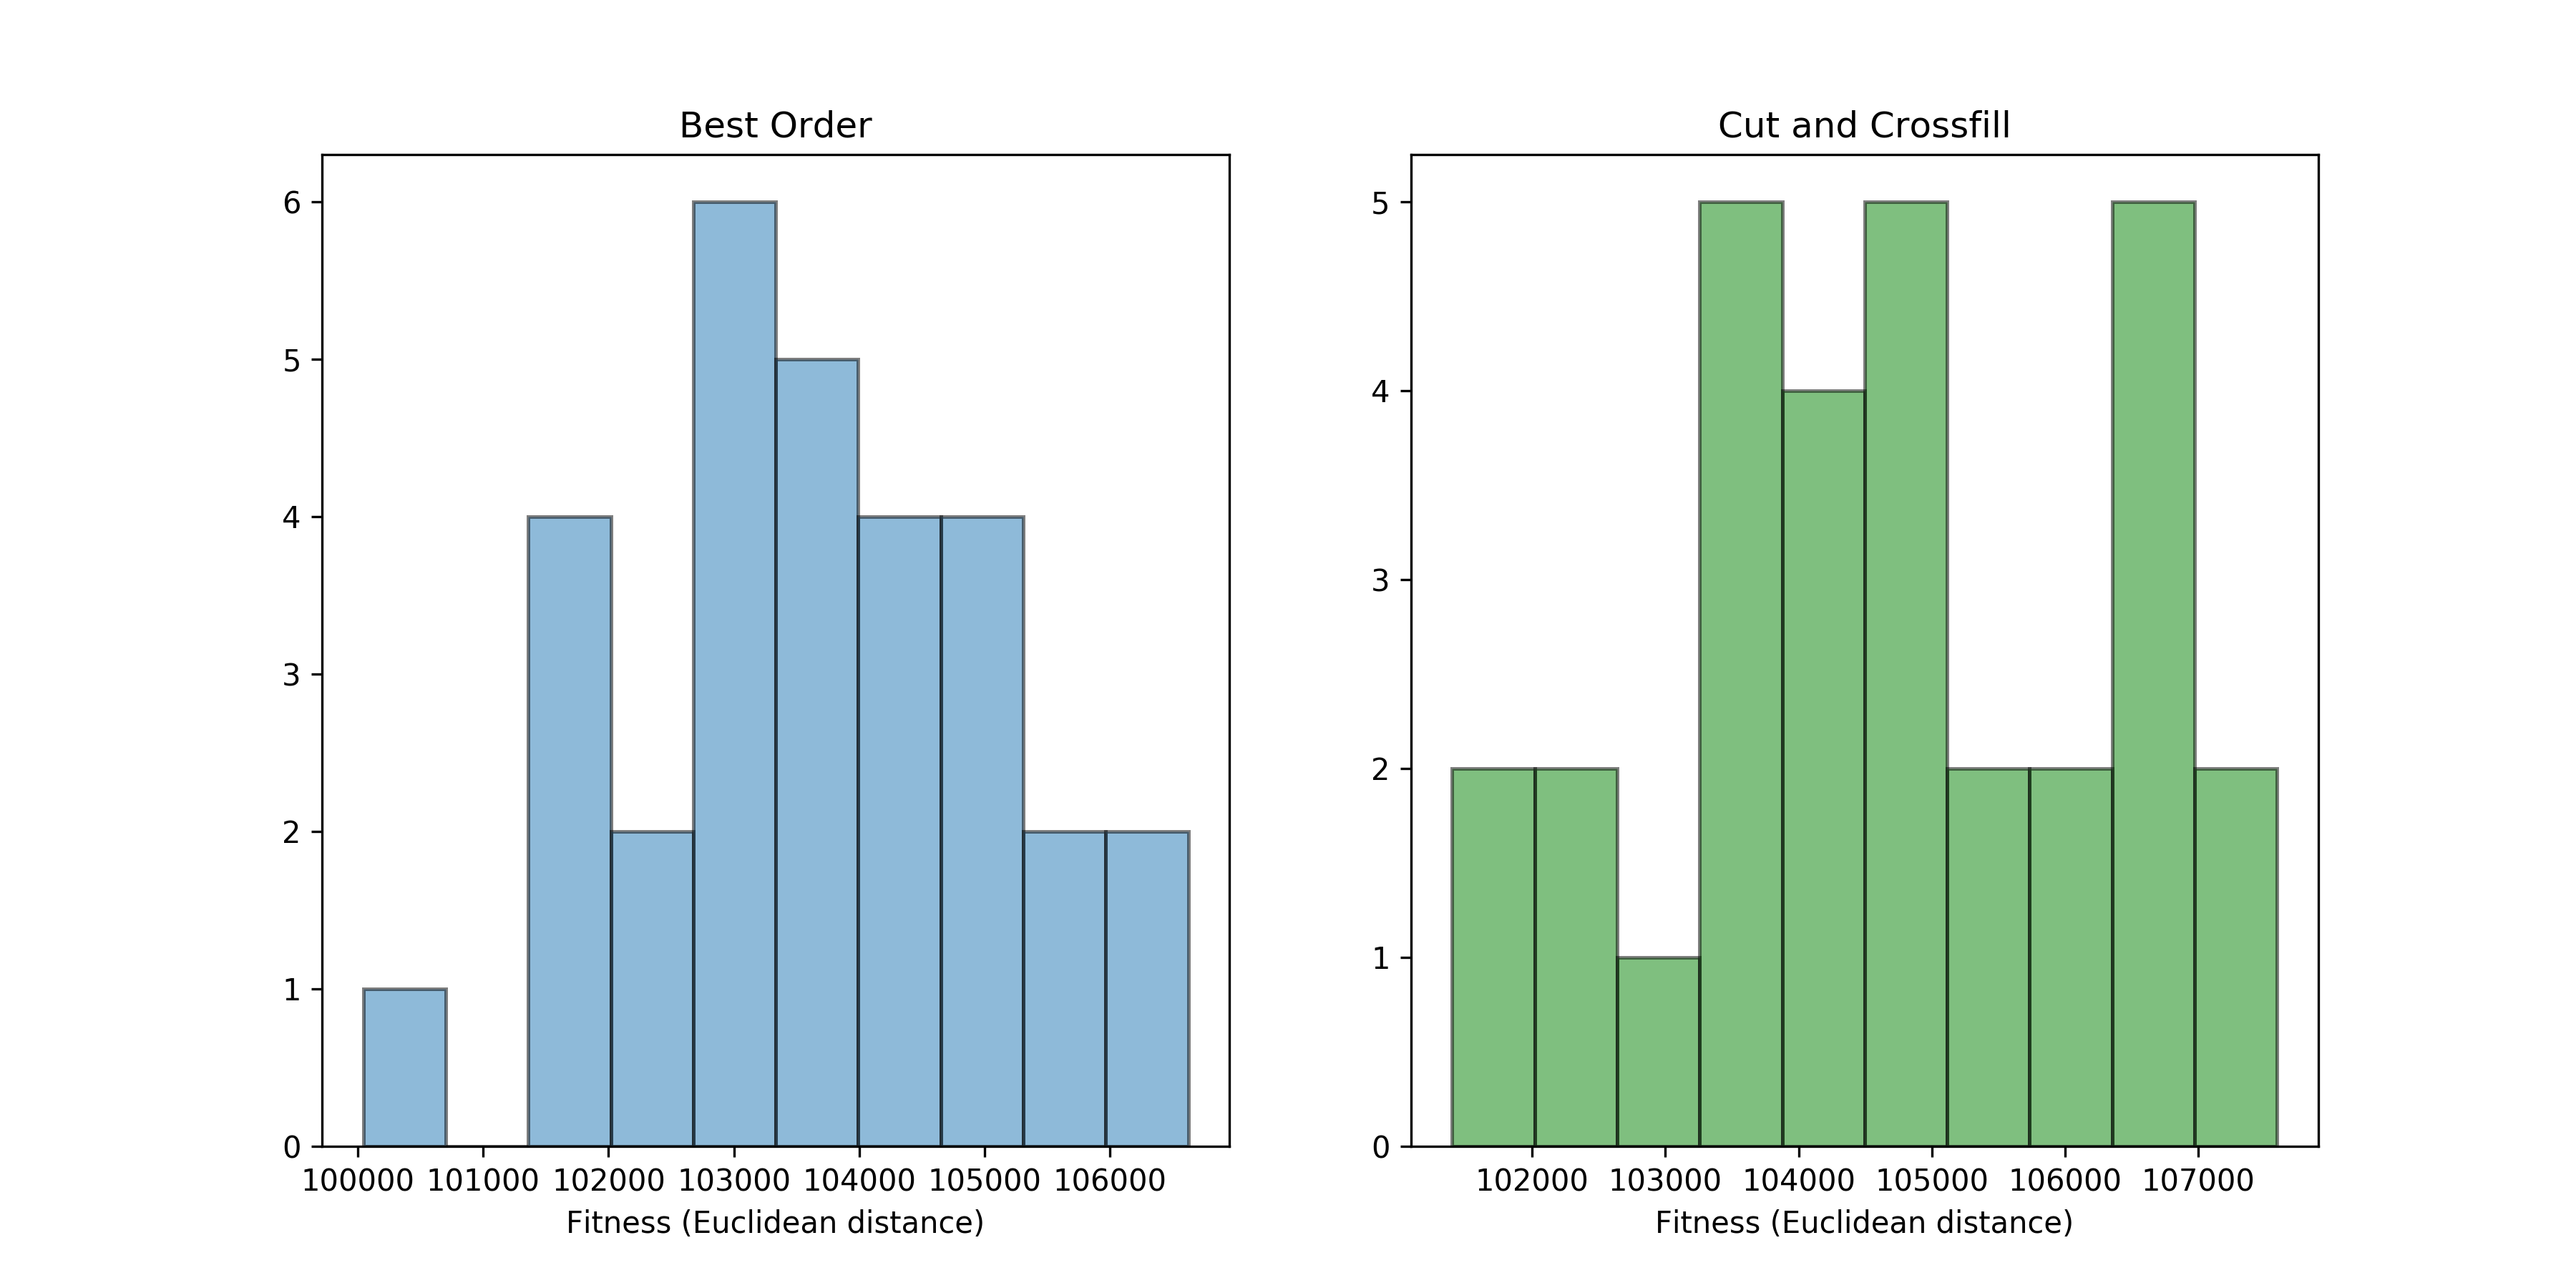
\includegraphics[width=\linewidth]{bocchist.png}}
\caption{Illustration of the distribution of samples of the best individual achieved in samples of thirty runs of each crossover type.}
\label{fig:bocchist}
\end{figure}

\subsection{Mutation}




Figure \ref{fig:mg} gives a clear indication of the performance of each mutation operator. There is a clear gap in the performance as evidenced by the non-overlapping range of samples. It is evident that the best performing mutation operators are cyclic and scramble, however we cannot make any conclusion as to which is better. Looking at the notched boxplots in Figure \ref{fig:bpm} we notice that, between cyclic and scramble, the confidence intervals and median are nearly the same. The scramble mutation has a slightly larger range in the right tail, but there is not enough information to determine whether or not this is statistically significant.

It is important to note that the resultant mean fitness of both cyclic and scramble is about 104,000. This 131\% of the optimum distance of 79,114. This result is acceptable to us, in that we have only calculated 1000 generations to achieve this result.

\begin{figure}[htbp]
\centering
\fbox{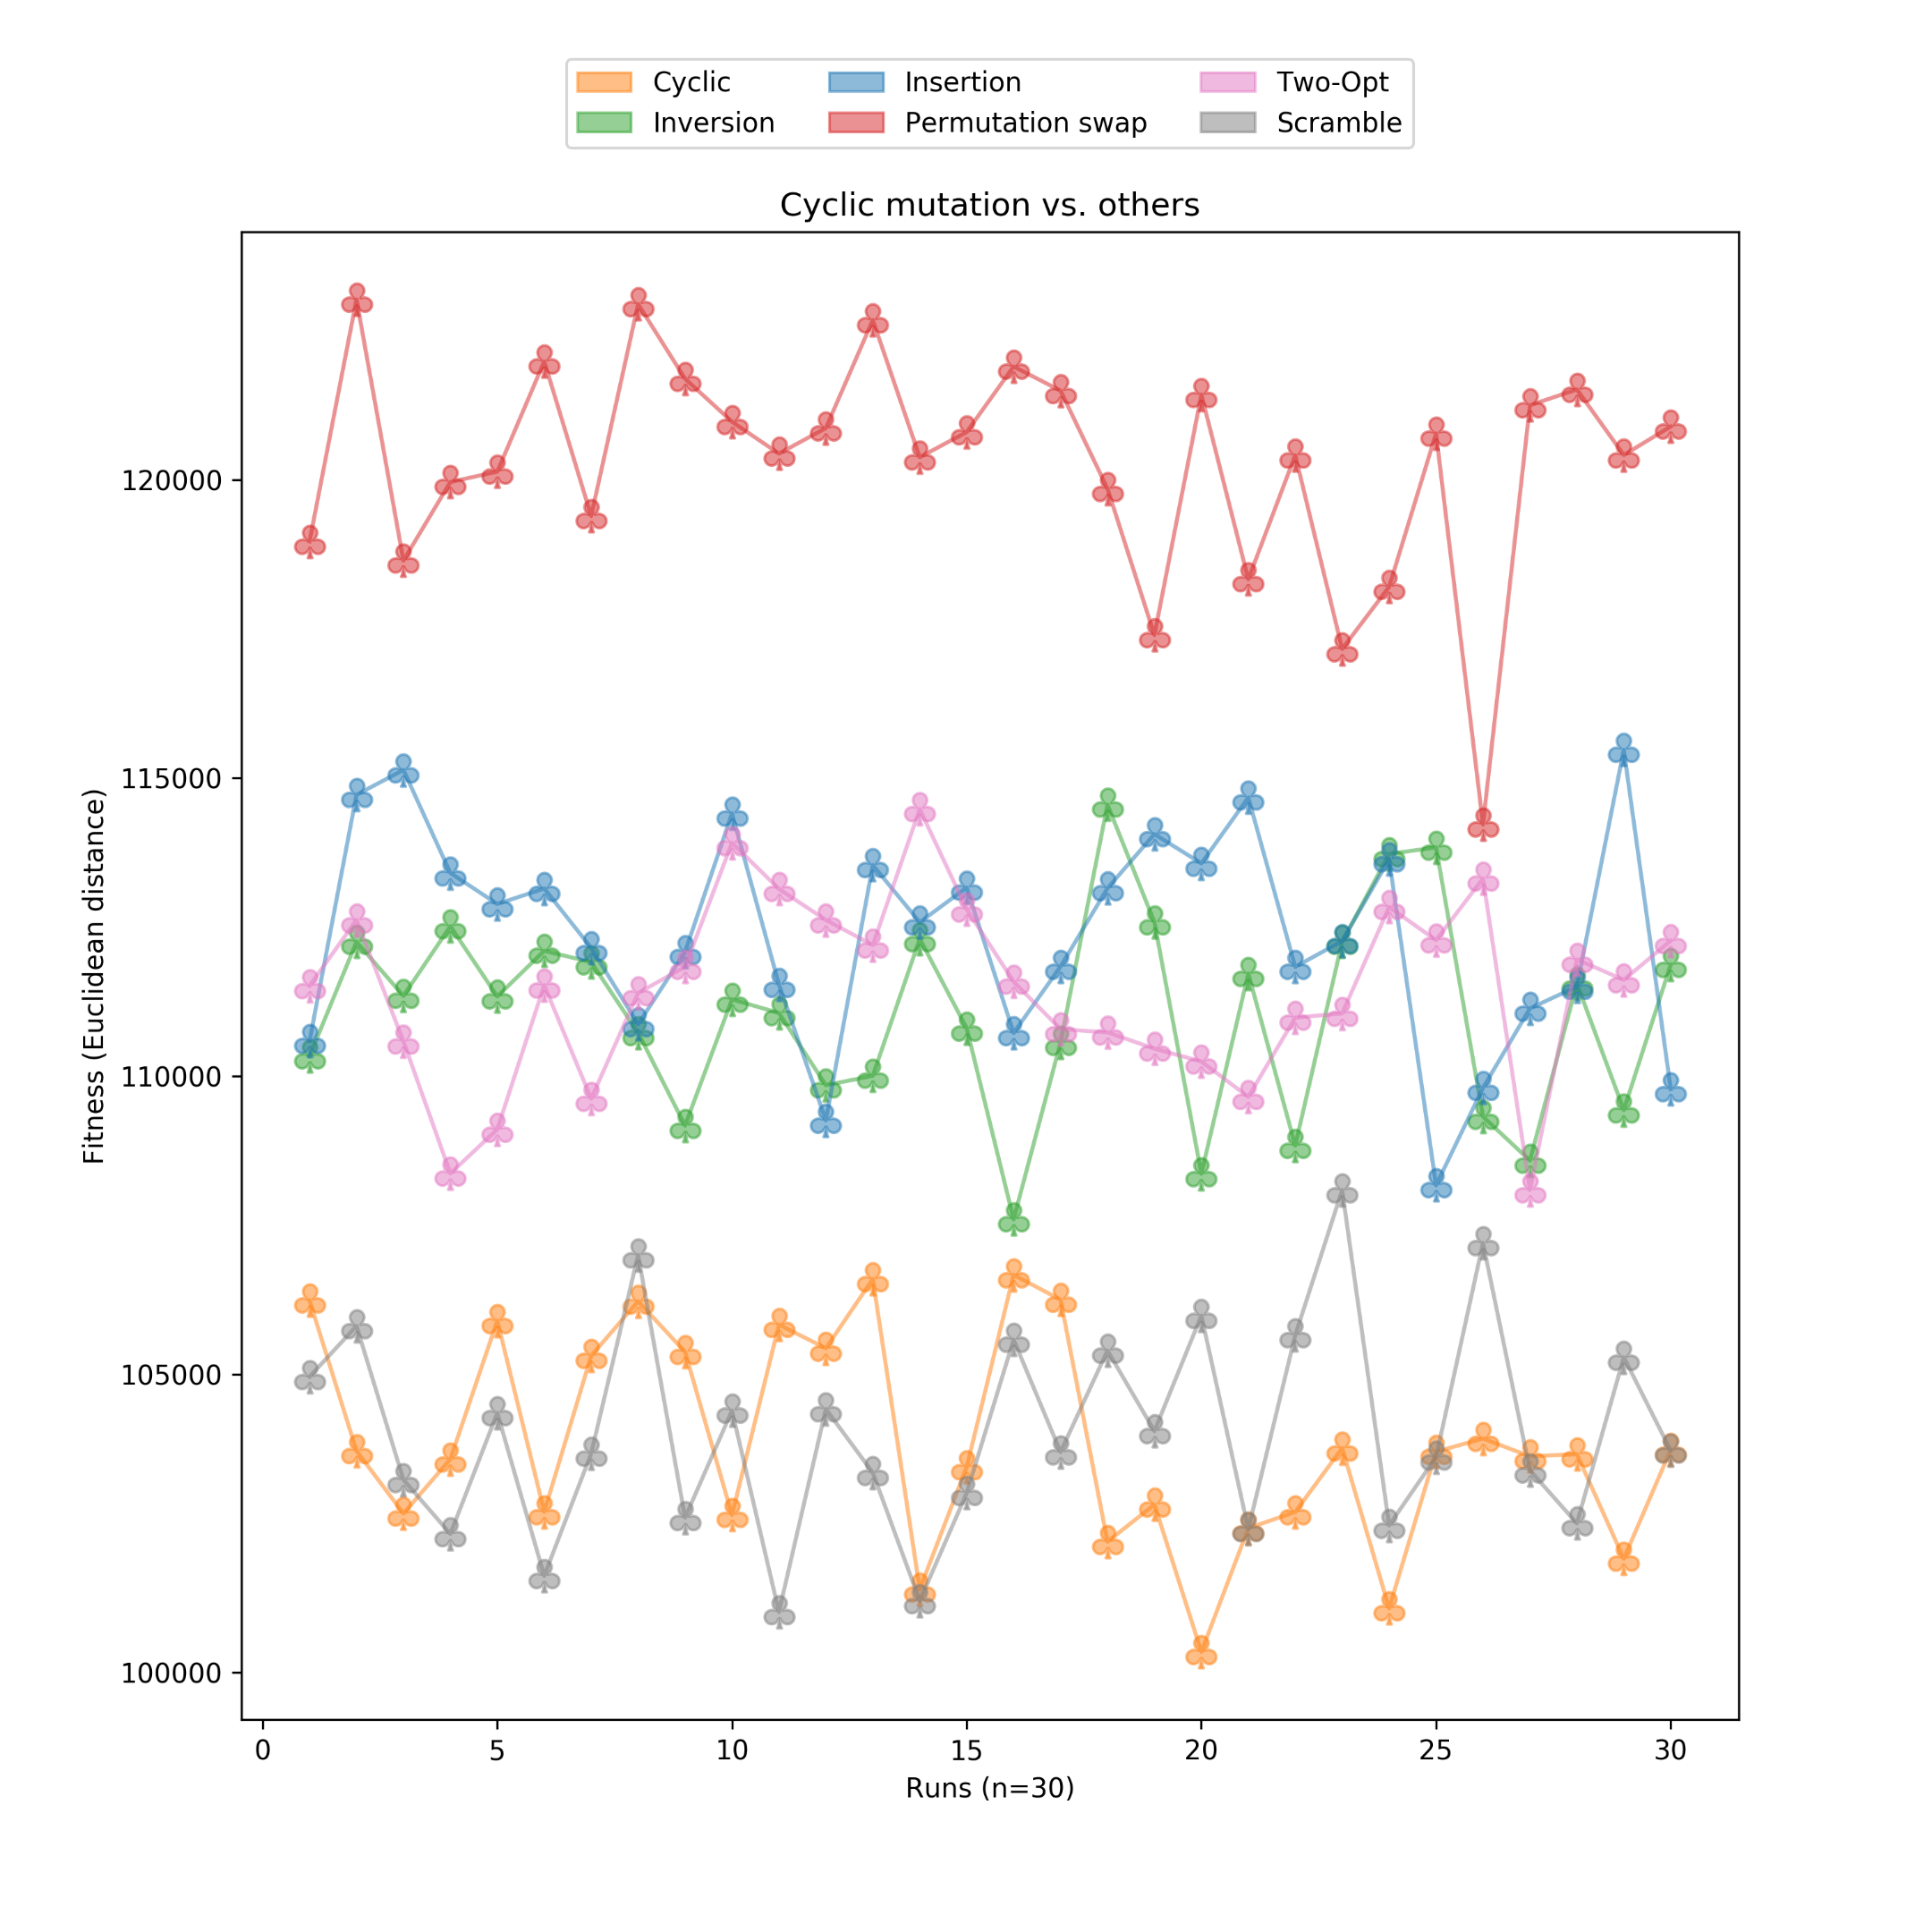
\includegraphics[width=\linewidth]{graphmut.png}}
\caption{Comparison of the mean best fitnesses produced by various types of mutation operators.}
\label{fig:mg}
\end{figure}

\begin{figure}[htbp]
\centering
\fbox{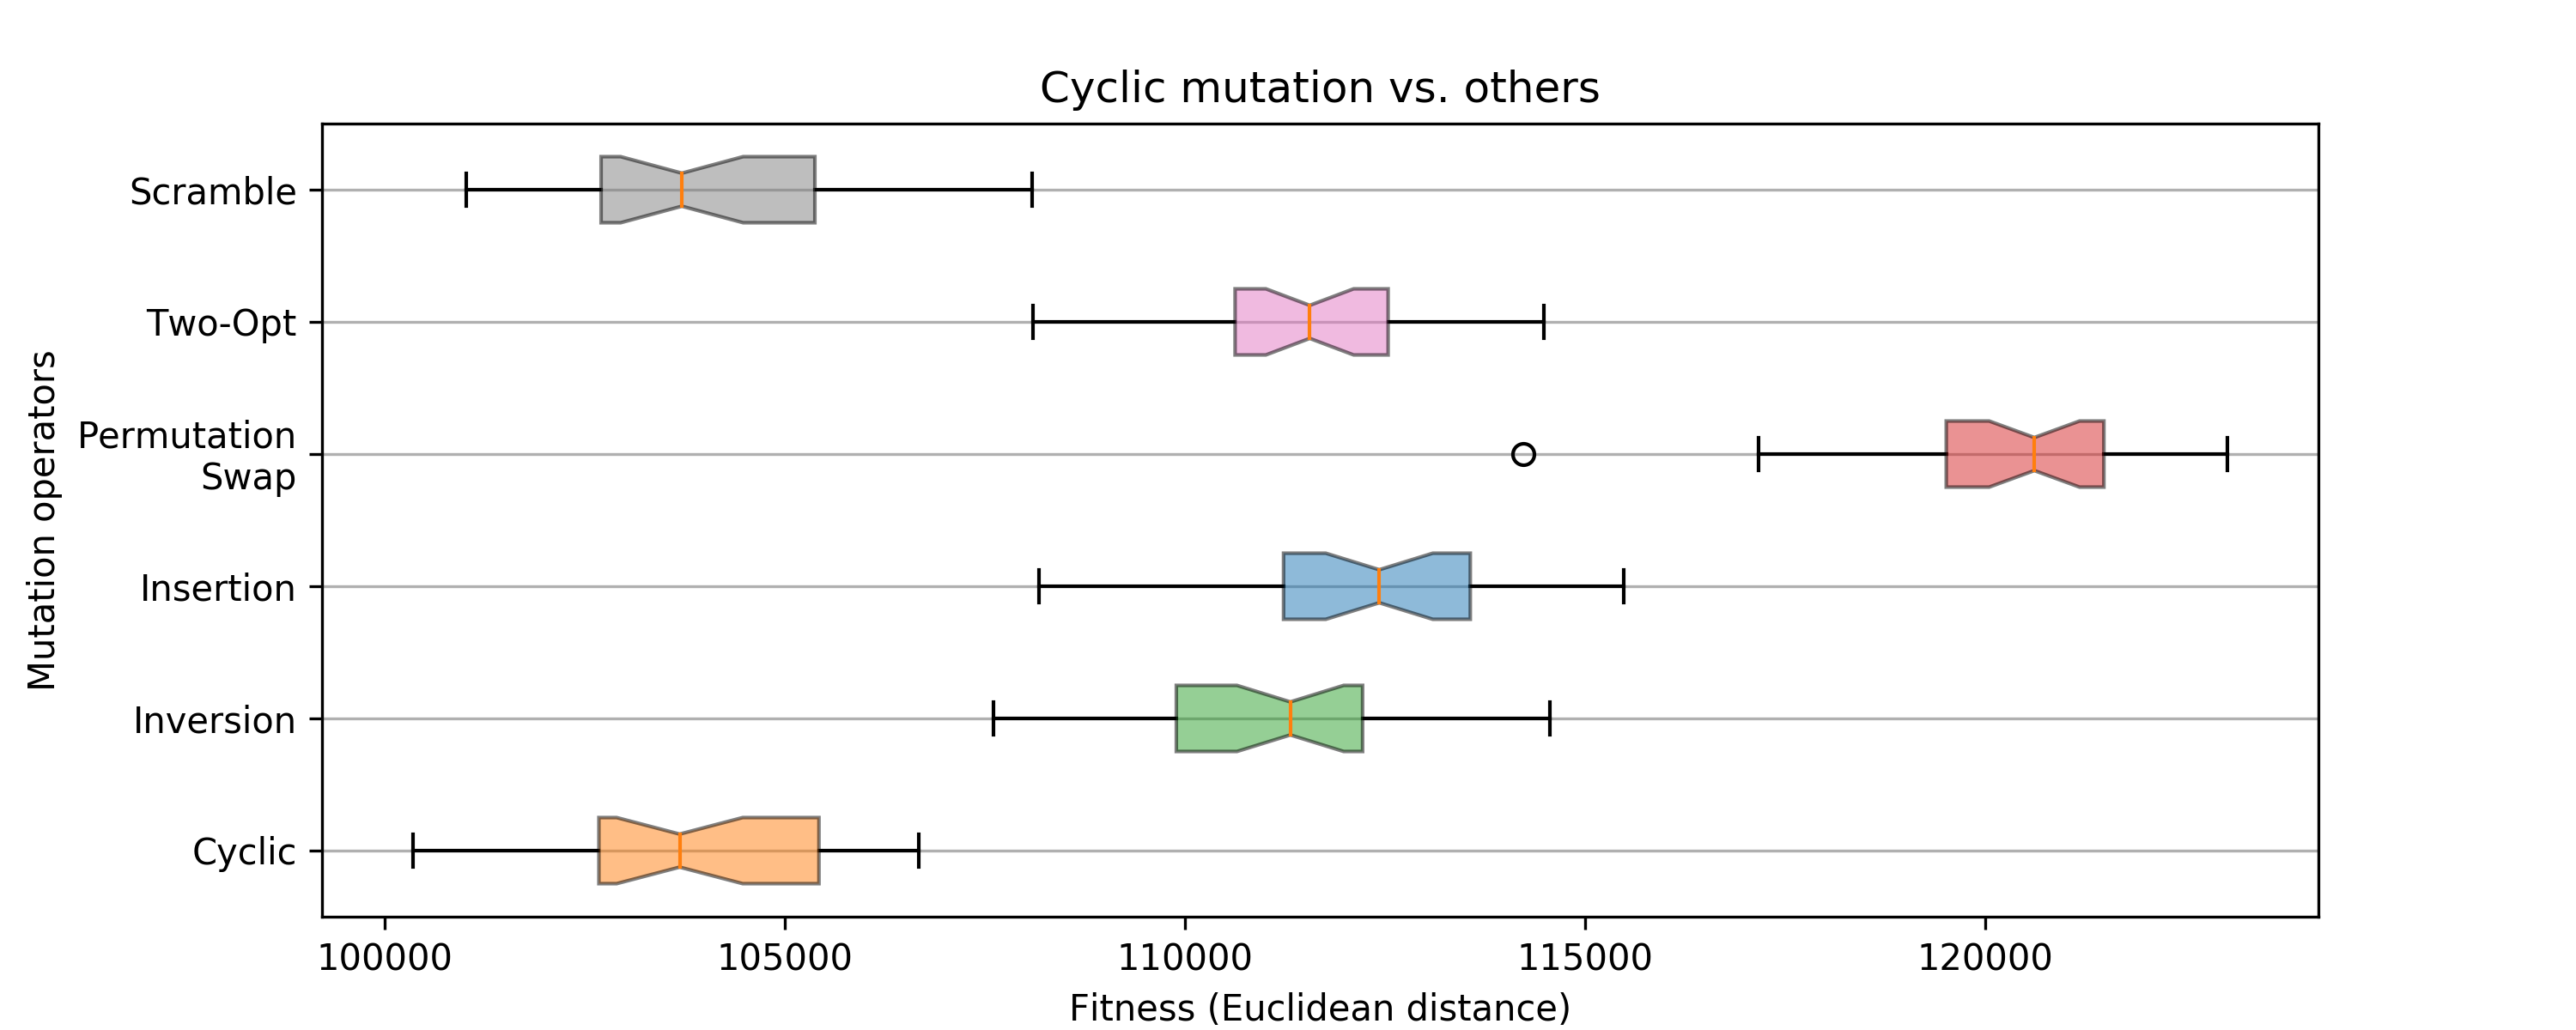
\includegraphics[width=\linewidth]{bpmutation.png}}
\caption{Notched boxplots of the distribution of best fitness for various types of mutation operators.}
\label{fig:bpm}
\end{figure}

As one might expect from Figure \ref{fig:bpm}, one-tailed Mann-Whitney-U tests reject the null hypothesis with an infinitesimally small p-value, with the exception of the comparison between scramble and cyclic mutation.

\subsection{Tuning Parameters}
The Python implementation described in this paper uses a number of parameters whose usage is explained in detail in the User Guide. Of these parameters, a select few are described in detail.

\textbf{box\_cutting\_points\_n} defines the number of crossover points chosen when using the best-order crossover operator. As we can see from Figure \ref{fig:boci}, varying this value only makes a minimal change to the boxplot. As expected, the Mann-Whitney-U test between all permutations of pairs of this set produces no rejection of the null hypothesis, with p-values near 0.50.
\begin{figure}[htbp]
\centering
\fbox{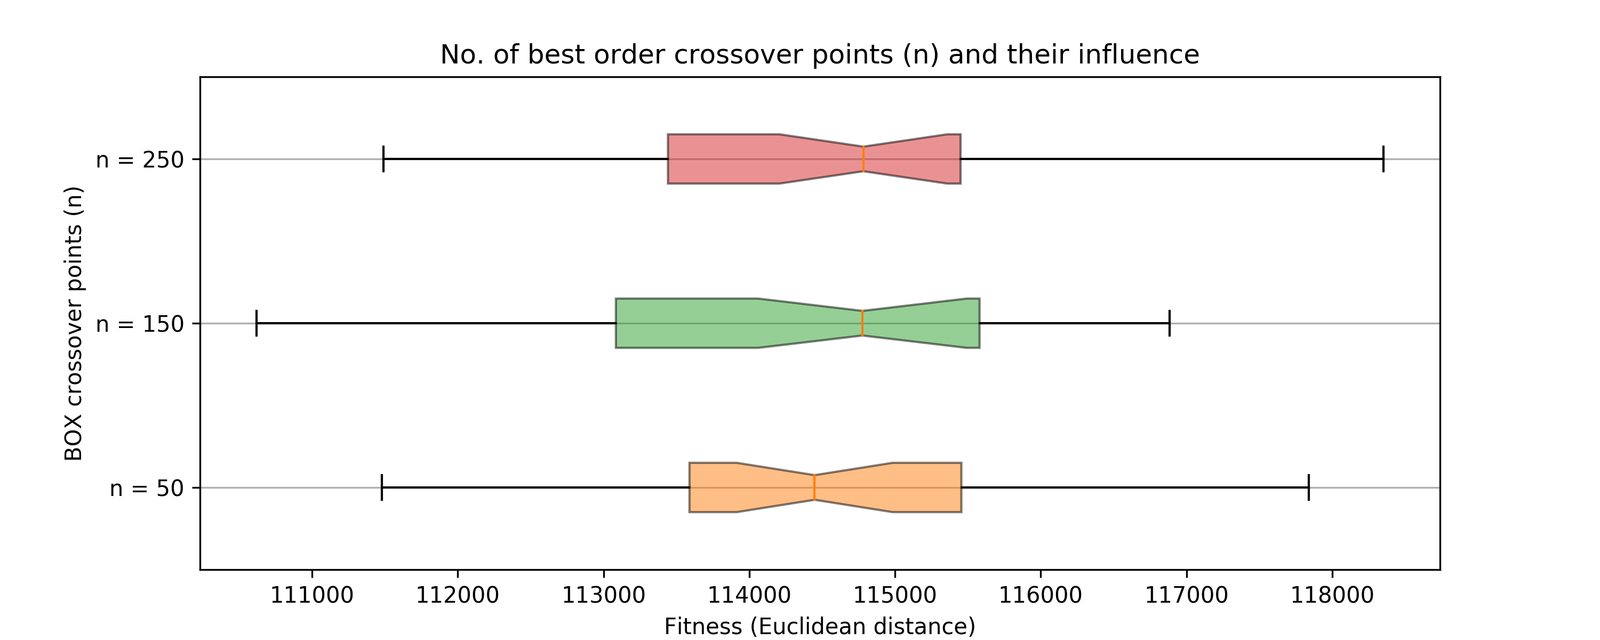
\includegraphics[width=\linewidth]{boci.png}}
\caption{Boxplots of three different parameters for the best-order crossover algorithm.}
\label{fig:boci}
\end{figure}

\textbf{kca\_k} defines the number of clusters that graph nodes should be split into. This parameter is usually specified as a proportion of the chromosome length. As the minuscule p-values for the parameter and the visualization in Figure \ref{fig:kcai} suggests,  more clusters lead to lower fitness values in the initial population. Therefore, the number of clusters has a statistically significant effect on the initial population fitness values that the algorithm starts out with.

\begin{figure}[htbp]
\centering
\fbox{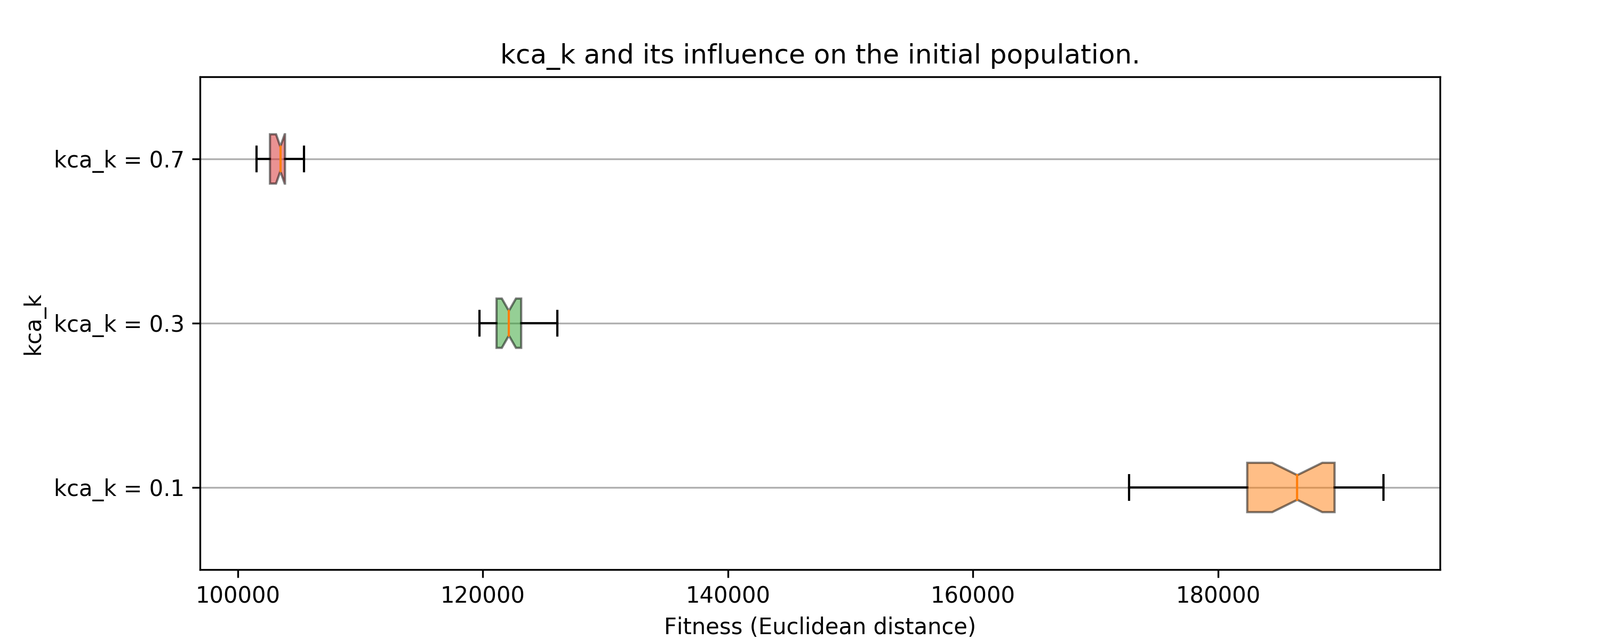
\includegraphics[width=\linewidth]{kcai.png}}
\caption{Boxplots of three different parameters for the number of clusters in the k-means algorithm.}
\label{fig:kcai}
\end{figure}

\textbf{kca\_iterations} describes the number of iterations performed in Step 3 of the k-means clustering algorithm outlined above. Note that, ideally Step 3 is performed until the clusters become constant between iterations. However, due to computational constraints, we refrain from doing so here. As the p-values and Figure \ref{fig:kci} indicate, there is insufficient evidence to claim that there is a statistically significant impact in varying levels of this parameter on the initial population’s fitness. However, one intriguing finding we obtained is that, as the above visualization indicates, as the numbers of iterations go up, the algorithm wounds up with worse fitness values, not better, which is the exact opposite of what we had hypothesized initially.
It is likely that more iterations forces the chromosome into an even deeper local minima, which would need an aggressive strategy or new type of mutation operator to exit. Certain alleles will be forced to be occupy a good, but not optimal, loci. It is the author's belief that it is prudent to limit this parameter to a very small number, otherwise a new strategy would be required to ascend the fitness landscape.

\begin{figure}[htbp]
\centering
\fbox{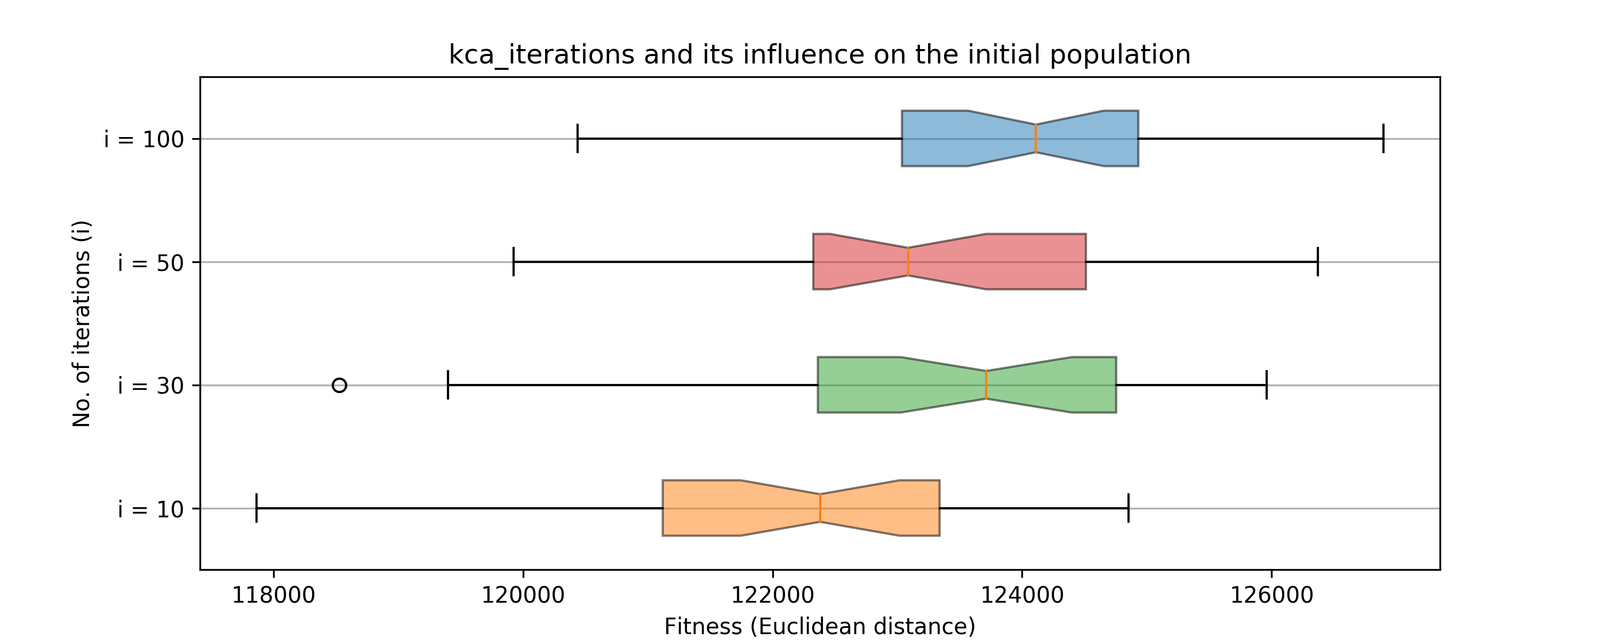
\includegraphics[width=\linewidth]{kci.png}}
\caption{Boxplots of three different parameters for the number of iterations in the k-means algorithm.}
\label{fig:kci}
\end{figure}


\subsection{Implementation Performance}
A variety of techniques were used to improve the performance, however more work needs to be done in this area. A complete understanding of how to use libraries like NumPy and Numba would speed up the algorithm considerably. The main focus of the program was on algorithms and ease-of-use, with the hope that multithreading would bridge the performance gap. This turned out to be a problem, since the main Python interpreter includes a \textit{Global Interpret Lock}, which only allows one thread to execute at a time. Without this constraint, multithreading would have been helpful in parallelising the calculations involved. Several attempts were made to use multiprocessing instead, but the overhead associated with this was not worth the effort. In many cases, the algorithm became slower. At other times, it overwhelmed the garbage collection of the Python interpreter by spawning many copies of the local memory spaces, only to immediately remove them as soon as the calculation had finished.

Constant time array look-ups are used wherever possible. The matrix describing the distances between all sets of nodes is generated and cached to a file to speed up subsequent runs. Recombination is the choke point of this algorithm, as best-order provides a description that depends on certain mathematical constraints on the sequence of cutting points on the chromosome. Unfortunately, the authors were unable to determine an iterative solution to the generation of cutting points. Instead random points were generated and tested against the constraints. Despite this, the recombination time is very reasonable, considering its complexity.

The k-means clustering algorithm also takes considerable time to run, however the cost is worth it. The reduction in the search space cuts several thousand years off of the computational time. There are libraries available to implement clustering algorithms, such as SciPy. The authors opted to write an implementation of k-means from scratch so that inferences could be made from the intermediary results.

\section{Conclusion}
After determining the optimal parameter set, each of the data sets were ran thirty times to determine the optimal results and the algorithmic run times. 


Given more time, considerable focus should be spent on determining a method to get a closer match to the optimal ordering of clusters. There is potential to use a cluster-boundary informed sub-segment swap to as a mutation operator to further optimize the algorithm. Raven's \textit{Biology}\cite{raven2001biology} describes the idea of \textit{transposons}, sub-segments of a chromosome that can move to a different neighborhood.

Reinforcement learning is possibly another avenue for optimizing this algorithm. The survivor selection can become probabilistic depending on whether or not the fitness value has plateaued. Using temporal-difference learning would be ideal for this, as it would let the algorithm decide when to change strategies. It may be possible to exit local minima with this method. More testing into these methods may be warranted.

\bigskip

% Bibliography
\bibliography{sample}

% Full bibliography added automatically for Optics Letters submissions; the following line will simply be ignored if submitting to other journals.
% Note that this extra page will not count against page length
\bibliographyfullrefs{sample}

%Manual citation list
%\begin{thebibliography}{1}
%\bibitem{Zhang:14}
%Y.~Zhang, S.~Qiao, L.~Sun, Q.~W. Shi, W.~Huang, %L.~Li, and Z.~Yang,
 % \enquote{Photoinduced active terahertz metamaterials with nanostructured
  %vanadium dioxide film deposited by sol-gel method,} Opt. Express \textbf{22},
  %11070--11078 (2014).
%\end{thebibliography}




\end{document}
